\documentclass[tikz,border=12pt]{standalone}
\usepackage{tikz}
\usepackage{amsmath}
\usepackage{amssymb}
\usepackage{xcolor}
\usetikzlibrary{shapes.geometric,arrows.meta,positioning,fit,backgrounds,calc}

\definecolor{inputBlue}{RGB}{208,228,245}
\definecolor{inputBorder}{RGB}{100,150,200}
\definecolor{svdGreen}{RGB}{200,230,200}
\definecolor{svdBorder}{RGB}{80,160,80}
\definecolor{mpYellow}{RGB}{255,242,160}
\definecolor{mpBorder}{RGB}{200,170,40}
\definecolor{assemblyPink}{RGB}{245,200,210}
\definecolor{assemblyBorder}{RGB}{190,80,100}
\definecolor{memGray}{RGB}{230,230,230}
\definecolor{memBorder}{RGB}{140,140,140}
\definecolor{arrowColor}{RGB}{60,60,60}

\tikzset{
  panel/.style={rounded corners=7pt, draw=#1, line width=1.5pt, inner sep=8pt},
  pbox/.style={draw=#1, fill=#1!30, rounded corners=5pt, line width=1pt,
    minimum width=2.0cm, minimum height=0.9cm, align=center, font=\small},
  rotbox/.style={draw=svdBorder, fill=svdGreen, rounded corners=3pt, line width=0.8pt,
    minimum width=3.0cm, minimum height=0.65cm, align=center, font=\scriptsize},
  mbox/.style={draw=memBorder, fill=memGray, rounded corners=3pt,
    minimum width=2.5cm, minimum height=0.5cm, align=center, font=\scriptsize},
  brainbox/.style={draw=gray!50, fill=gray!12, rounded corners=3pt,
    minimum width=1.4cm, minimum height=1.8cm, align=center, font=\tiny},
  arr/.style={-{Stealth[length=5pt,width=4pt]}, line width=1.1pt, color=arrowColor},
  sarr/.style={-{Stealth[length=4pt,width=3pt]}, line width=0.8pt, color=arrowColor},
  darr/.style={-{Stealth[length=4pt,width=3pt]}, line width=0.8pt, color=arrowColor, dashed},
}

\begin{document}
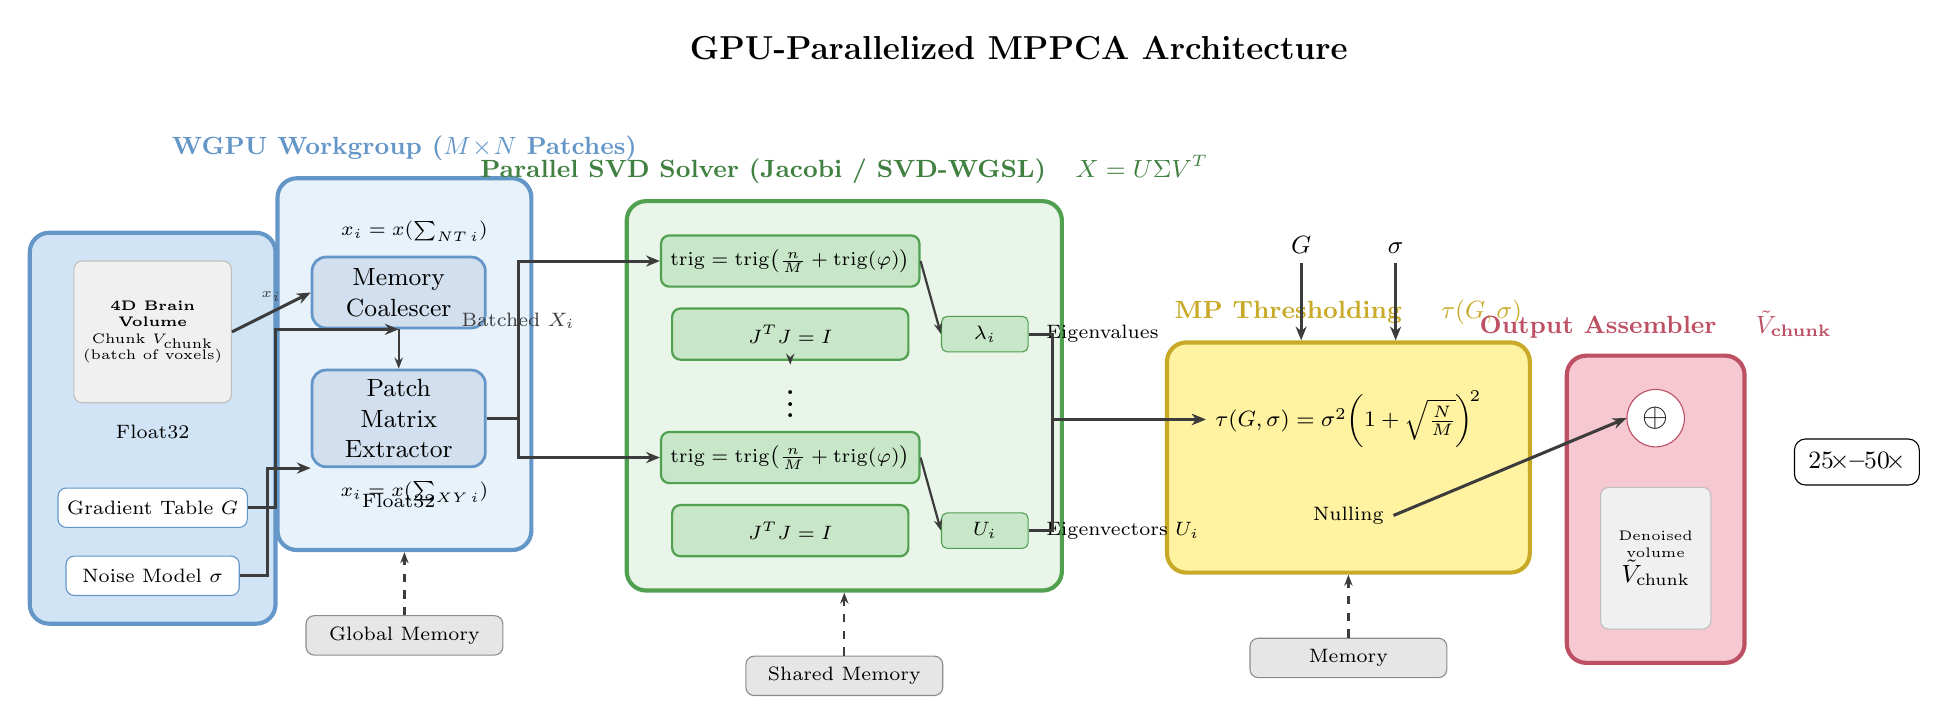
\begin{tikzpicture}[node distance=0.5cm and 0.5cm]

% TITLE
\node[font=\large\bfseries] (TITLE) at (11,0.8)
  {GPU-Parallelized \textbf{MPPCA} Architecture};

%% COLUMN 1 - INPUTS
\node[brainbox] (brain) at (0,-2.8)
  {\textbf{4D Brain}\\\textbf{Volume}\\Chunk $V_{\text{chunk}}$\\(batch of voxels)};
\node[font=\scriptsize, below=0.15cm of brain] (f32a) {Float32};
\node[draw=inputBorder, fill=white, rounded corners=3pt, font=\scriptsize,
      minimum width=2.2cm, minimum height=0.5cm, align=center,
      below=0.5cm of f32a] (gradT) {Gradient Table $G$};
\node[draw=inputBorder, fill=white, rounded corners=3pt, font=\scriptsize,
      minimum width=2.2cm, minimum height=0.5cm, align=center,
      below=0.35cm of gradT] (noiseM) {Noise Model $\sigma$};
\begin{scope}[on background layer]
  \node[panel=inputBorder, fill=inputBlue,
        fit=(brain)(f32a)(gradT)(noiseM), inner sep=10pt] (P1) {};
\end{scope}

%% COLUMN 2 - WGPU WORKGROUP
\node[pbox=inputBorder, minimum width=2.2cm,
      right=1.0cm of brain, yshift=0.5cm] (memC) {Memory\\Coalescer};
\node[pbox=inputBorder, minimum width=2.2cm,
      below=0.5cm of memC] (patchE) {Patch\\Matrix\\Extractor};
\node[font=\scriptsize, below=0.2cm of patchE] (f32b) {Float32};
\node[font=\scriptsize, above=0.05cm of memC, xshift=0.2cm] (xi1eq)
  {$x_i = x(\sum_{NT\,i})$};
\node[font=\scriptsize, below=0.05cm of patchE, xshift=0.2cm] (xi2eq)
  {$x_i = x(\sum_{XY\,i})$};
\begin{scope}[on background layer]
  \node[panel=inputBorder, fill=inputBlue!50,
        fit=(memC)(patchE)(f32b)(xi1eq)(xi2eq), inner sep=12pt] (P2) {};
\end{scope}
\node[font=\small\bfseries, text=inputBorder, above=2pt of P2.north, anchor=south]
  {WGPU Workgroup ($M\!\times\!N$ Patches)};

%% COLUMN 3 - PARALLEL SVD SOLVER
\node[rotbox, right=2.2cm of memC, yshift=0.4cm] (rot1)
  {$\mathrm{trig}=\mathrm{trig}\!\left(\tfrac{n}{M}+\mathrm{trig}(\varphi)\right)$};
\node[rotbox, below=0.25cm of rot1] (jj1) {$J^TJ = I$};
\node[font=\Large, below=0.05cm of jj1] (vdots) {$\vdots$};
\node[rotbox, below=0.05cm of vdots] (rot2)
  {$\mathrm{trig}=\mathrm{trig}\!\left(\tfrac{n}{M}+\mathrm{trig}(\varphi)\right)$};
\node[rotbox, below=0.25cm of rot2] (jj2) {$J^TJ = I$};

\node[draw=svdBorder, fill=svdGreen, rounded corners=2pt, font=\scriptsize,
      minimum width=1.1cm, minimum height=0.45cm,
      right=0.4cm of jj1] (ev1) {$\lambda_i$};
\node[font=\scriptsize, right=0.1cm of ev1] {Eigenvalues};

\node[draw=svdBorder, fill=svdGreen, rounded corners=2pt, font=\scriptsize,
      minimum width=1.1cm, minimum height=0.45cm,
      right=0.4cm of jj2] (ev2) {$U_i$};
\node[font=\scriptsize, right=0.1cm of ev2] {Eigenvectors $U_i$};

\begin{scope}[on background layer]
  \node[panel=svdBorder, fill=svdGreen!40,
        fit=(rot1)(jj1)(vdots)(rot2)(jj2)(ev1)(ev2), inner sep=12pt] (P3) {};
\end{scope}
\node[font=\small\bfseries, text=svdBorder!80!black,
      above=2pt of P3.north, anchor=south, align=center]
  {Parallel SVD Solver (Jacobi / SVD-WGSL)\quad $X = U\Sigma V^T$};

%% COLUMN 4 - MP THRESHOLDING
\node[font=\footnotesize, align=center,
      right=1.8cm of P3.east, yshift=-0.3cm] (tauF)
  {$\tau(G,\sigma)=\sigma^2\!\left(1+\sqrt{\tfrac{N}{M}}\right)^{\!2}$};
\node[font=\scriptsize, below=0.5cm of tauF] (nulling) {Nulling};
\node[font=\small, above=1.5cm of tauF, xshift=-0.6cm] (Gin) {$G$};
\node[font=\small, above=1.5cm of tauF, xshift=0.6cm] (Sig) {$\sigma$};

\begin{scope}[on background layer]
  \node[panel=mpBorder, fill=mpYellow,
        fit=(tauF)(nulling), inner sep=14pt] (P4) {};
\end{scope}
\node[font=\small\bfseries, text=mpBorder,
      above=2pt of P4.north, anchor=south, align=center]
  {MP Thresholding \quad $\tau(G,\sigma)$};

%% COLUMN 5 - OUTPUT ASSEMBLER
\node[draw=assemblyBorder, circle, fill=white, inner sep=3pt, font=\large,
      right=1.2cm of P4.east, yshift=0.5cm] (cplus) {$\oplus$};
\node[brainbox, below=0.5cm of cplus] (brainOut)
  {Denoised\\volume\\\small $\tilde{V}_{\text{chunk}}$};

\begin{scope}[on background layer]
  \node[panel=assemblyBorder, fill=assemblyPink,
        fit=(cplus)(brainOut), inner sep=12pt] (P5) {};
\end{scope}
\node[font=\small\bfseries, text=assemblyBorder,
      above=2pt of P5.north, anchor=south, align=center]
  {Output Assembler \quad $\tilde{V}_{\text{chunk}}$};

% Speedup badge
\node[draw=black, fill=white, rounded corners=4pt,
      font=\small\bfseries, inner sep=5pt,
      right=0.6cm of P5.east, yshift=0.6cm]
  {$25\!\times$--$50\!\times$};

%% MEMORY BOXES
\node[mbox, below=0.8cm of P2.south] (globM) {Global Memory};
\node[mbox, below=0.8cm of P3.south] (sharedM) {Shared Memory};
\node[mbox, below=0.8cm of P4.south] (outM) {Memory};

%% ARROWS
\draw[arr] (brain.east) -- (memC.west)
  node[font=\tiny, midway, above] {$x_i$};
\draw[arr] (gradT.east) -- ++(0.35,0) |- (memC.south);
\draw[arr] (noiseM.east) -- ++(0.35,0) |- (patchE.south west);
\draw[sarr] (memC.south) -- (patchE.north);

\draw[arr] (patchE.east) -- ++(0.4,0) |- (rot1.west)
  node[font=\scriptsize, near start, above] {Batched $X_i$};
\draw[arr] (patchE.east) -- ++(0.4,0) |- (rot2.west);

\draw[sarr] (rot1.east) -- (ev1.west);
\draw[sarr] (rot2.east) -- (ev2.west);
\draw[sarr] (jj1) -- (vdots);

\draw[arr] (ev1.east) -- ++(0.3,0) |- (tauF.west);
\draw[arr] (ev2.east) -- ++(0.3,0) |- (tauF.west);

\draw[arr] (Gin.south) -- (P4.north -| Gin);
\draw[arr] (Sig.south) -- (P4.north -| Sig);

\draw[arr] (nulling.east) -- (cplus.west);

\draw[darr] (globM.north) -- (P2.south);
\draw[darr] (sharedM.north) -- (P3.south);
\draw[darr] (outM.north) -- (P4.south);

\end{tikzpicture}
\end{document}
